% !TEX root = ../../ThesisGchatzi.tex

\graphicspath{{Papers/SIGSpatial2017/}{Papers/SIGSpatial2018/}}

\section{Hybrid Query Variants}
\label{sec:query_types}

Next, we outline different hybrid similarity search and join query variants, combining spatial distance with time series similarity.

\subsection{Similarity Search}
\label{subsec:sim_serach_prob}
We are interested in hybrid similarity search queries on geolocated time series, i.e., queries that retrieve search results based on both spatial distance and time series distance. In these queries, a geolocated time series $T_q$ is given as a reference, and the goal is to identify similar time series to $T_q$, based on both spatial distance and time series distance. Different query variants can be derived. First, the query condition can be applied on each distance independently or on the hybrid distance defined in Section~\ref{subsec:index_pruning}. Second, the condition can be a boolean filter (i.e., retrieve all geolocated time series with distance lower than $\theta$) or a top-$k$ filter (i.e., retrieve the $k$ geolocated time series having the smallest distance). These lead to the hybrid query variants listed in Table \ref{tab:query_types} and outlined below:

\begin{itemize}
 \item $Q_{bb}(T_q, \theta_{sp}, \theta_{ts})$. This query applies two individual boolean filters. It retrieves each time series $T$ having $dist_{sp}(T_q, T) \leq \theta_{sp}$ and $dist_{ts}(T_q, T) \leq \theta_{ts}$. In other words, it retrieves all time series that are located within a radius $\theta_{sp} \cdot maxDist_{sp}$ from $T_q$'s location and their time series dissimilarity to $T_q$ is at most $\theta_{ts} \cdot maxDist_{ts}$.
 \item $Q_{kb}(T_q, k, \theta_{ts})$. This query retrieves the $k$ time series closest to $T_q$'s location also having $dist_{ts}(T_q, T) \leq \theta_{ts}$.
 \item $Q_{bk}(T_q, \theta_{sp}, k)$. This query retrieves the $k$ most similar time series to $T_q$ which are also located within distance $\theta_{sp} \cdot maxDist_{sp}$ from $T_q$'s location.
 \item $Q_{hb}(T_q, \theta_h, \gamma)$. This query retrieves all time series having hybrid distance to $T_q$ at most $\theta_h$, i.e., $dist_h(T_q, T) \leq \theta_h$.
 \item $Q_{hk}(T_q, k, \gamma)$. This query retrieves the $k$ time series with the smallest hybrid distance $dist_h(T_q, T)$ to $T_q$.
\end{itemize}

\begin{table}[!ht]
 \centering
 \caption{Similarity search query variants.}
 \vspace{-10pt}
 \begin{small}
 \begin{tabular}{c c c}
  \toprule
  Query Variant & Spatial Filter & Time Series Filter \\
  \midrule
  $Q_{bb}$ & boolean ($\theta_{sp}$) & boolean ($\theta_{ts}$) \\
  $Q_{kb}$ & top-$k$ & boolean ($\theta_{ts}$) \\
  $Q_{bk}$ & boolean ($\theta_{sp}$) & top-$k$ \\
  $Q_{hb}$ & \multicolumn{2}{c}{boolean ($\theta_{h}$)} \\
  $Q_{hk}$ & \multicolumn{2}{c}{top-$k$} \\
  \bottomrule
 \end{tabular}
 \end{small}
 \label{tab:query_types}
\end{table}

\begin{figure}[!tb]
 \centering
 \subfloat[$Q_{bb}(T_q, \theta_{sp}, \theta_{ts})$]{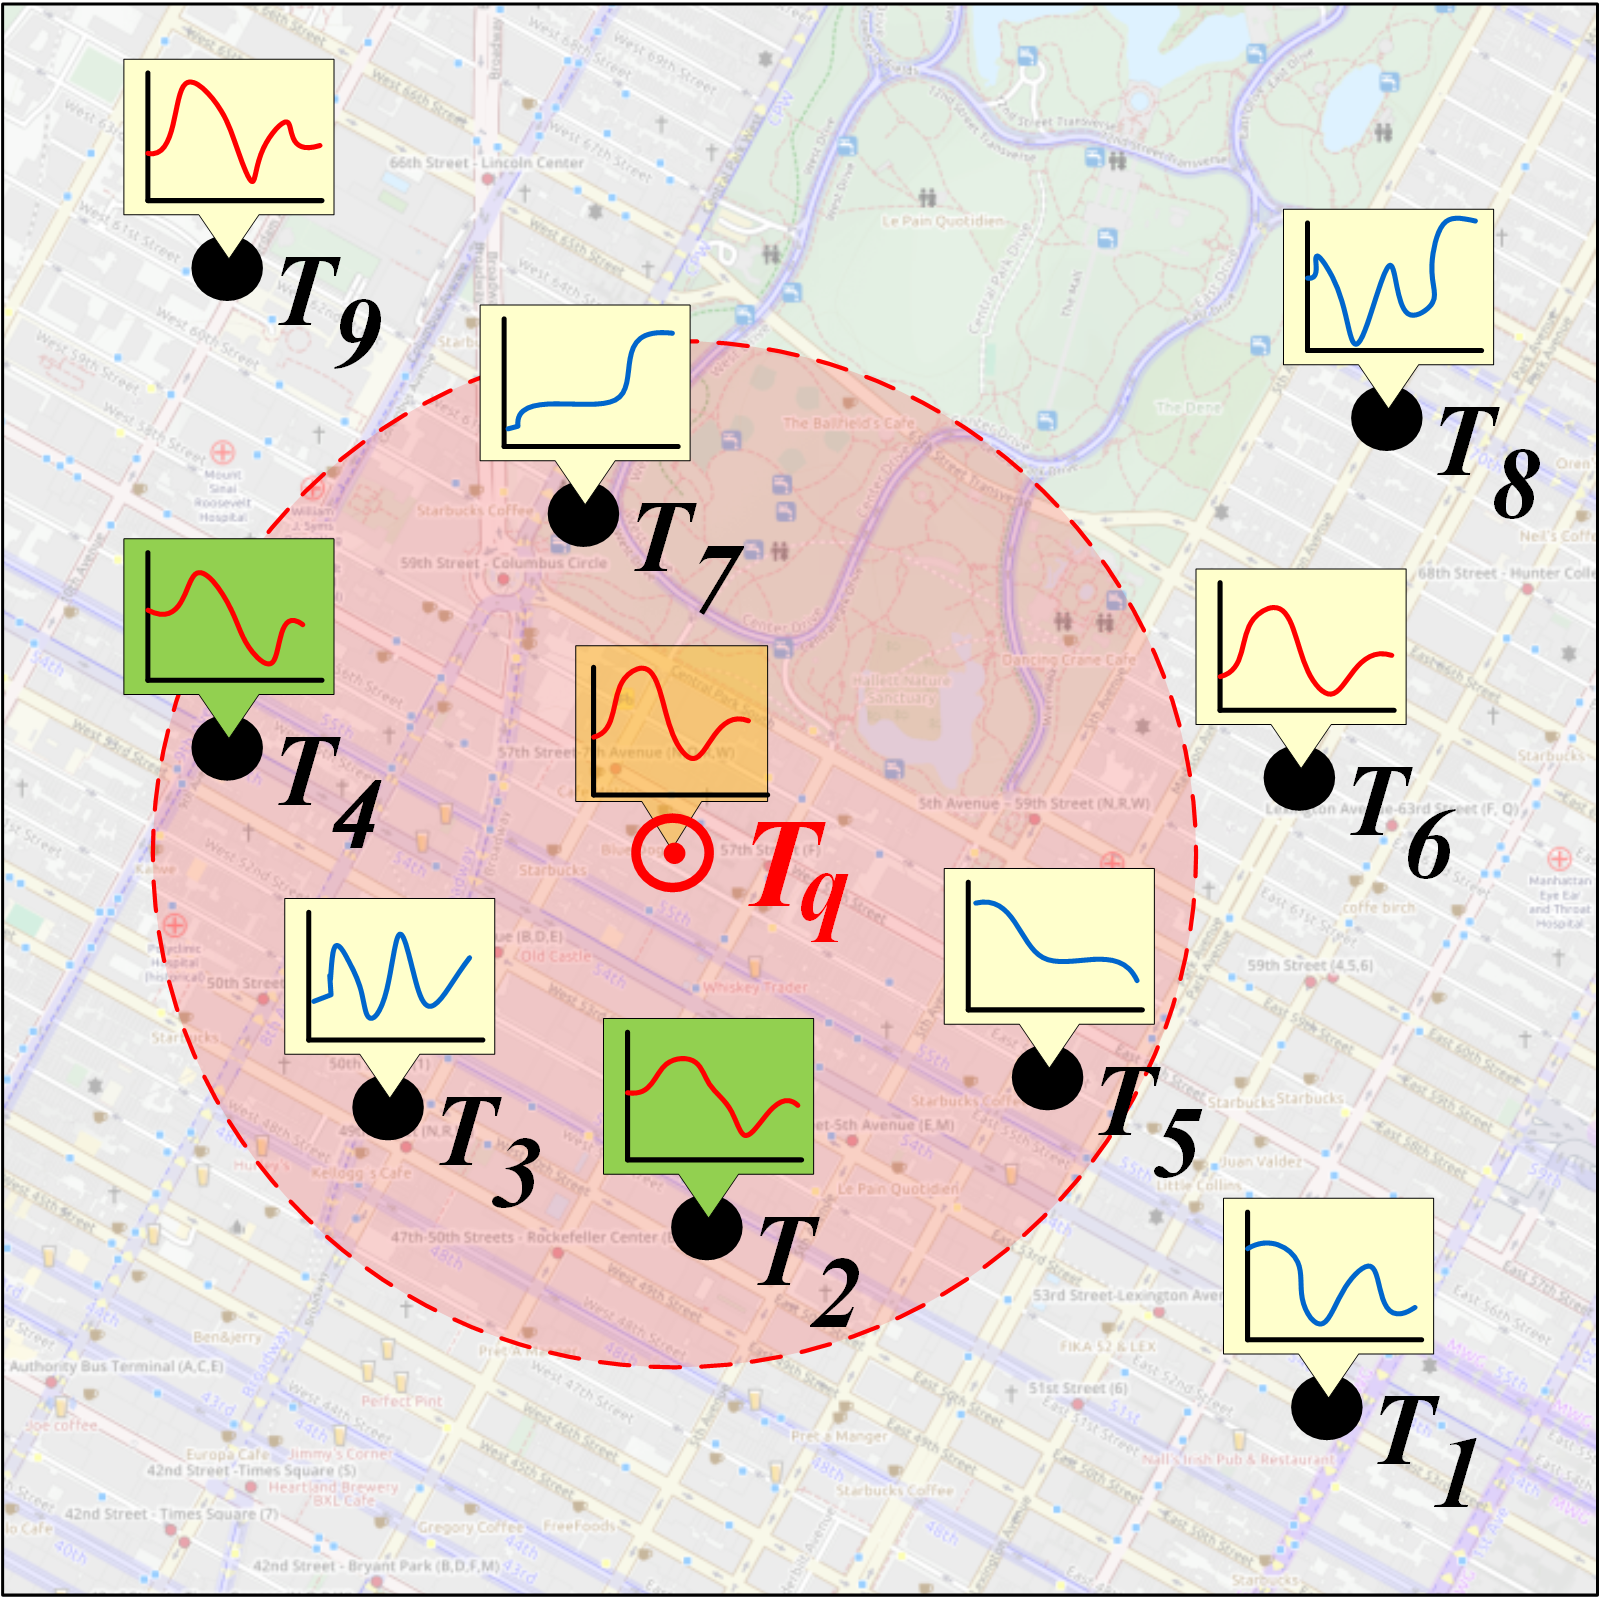
\includegraphics[width=0.3\textwidth]{figures/query_bb.png}\label{subfig:example_queries_bb}}
 \qquad
 \subfloat[$Q_{kb}(T_q, k, \theta_{ts})$]{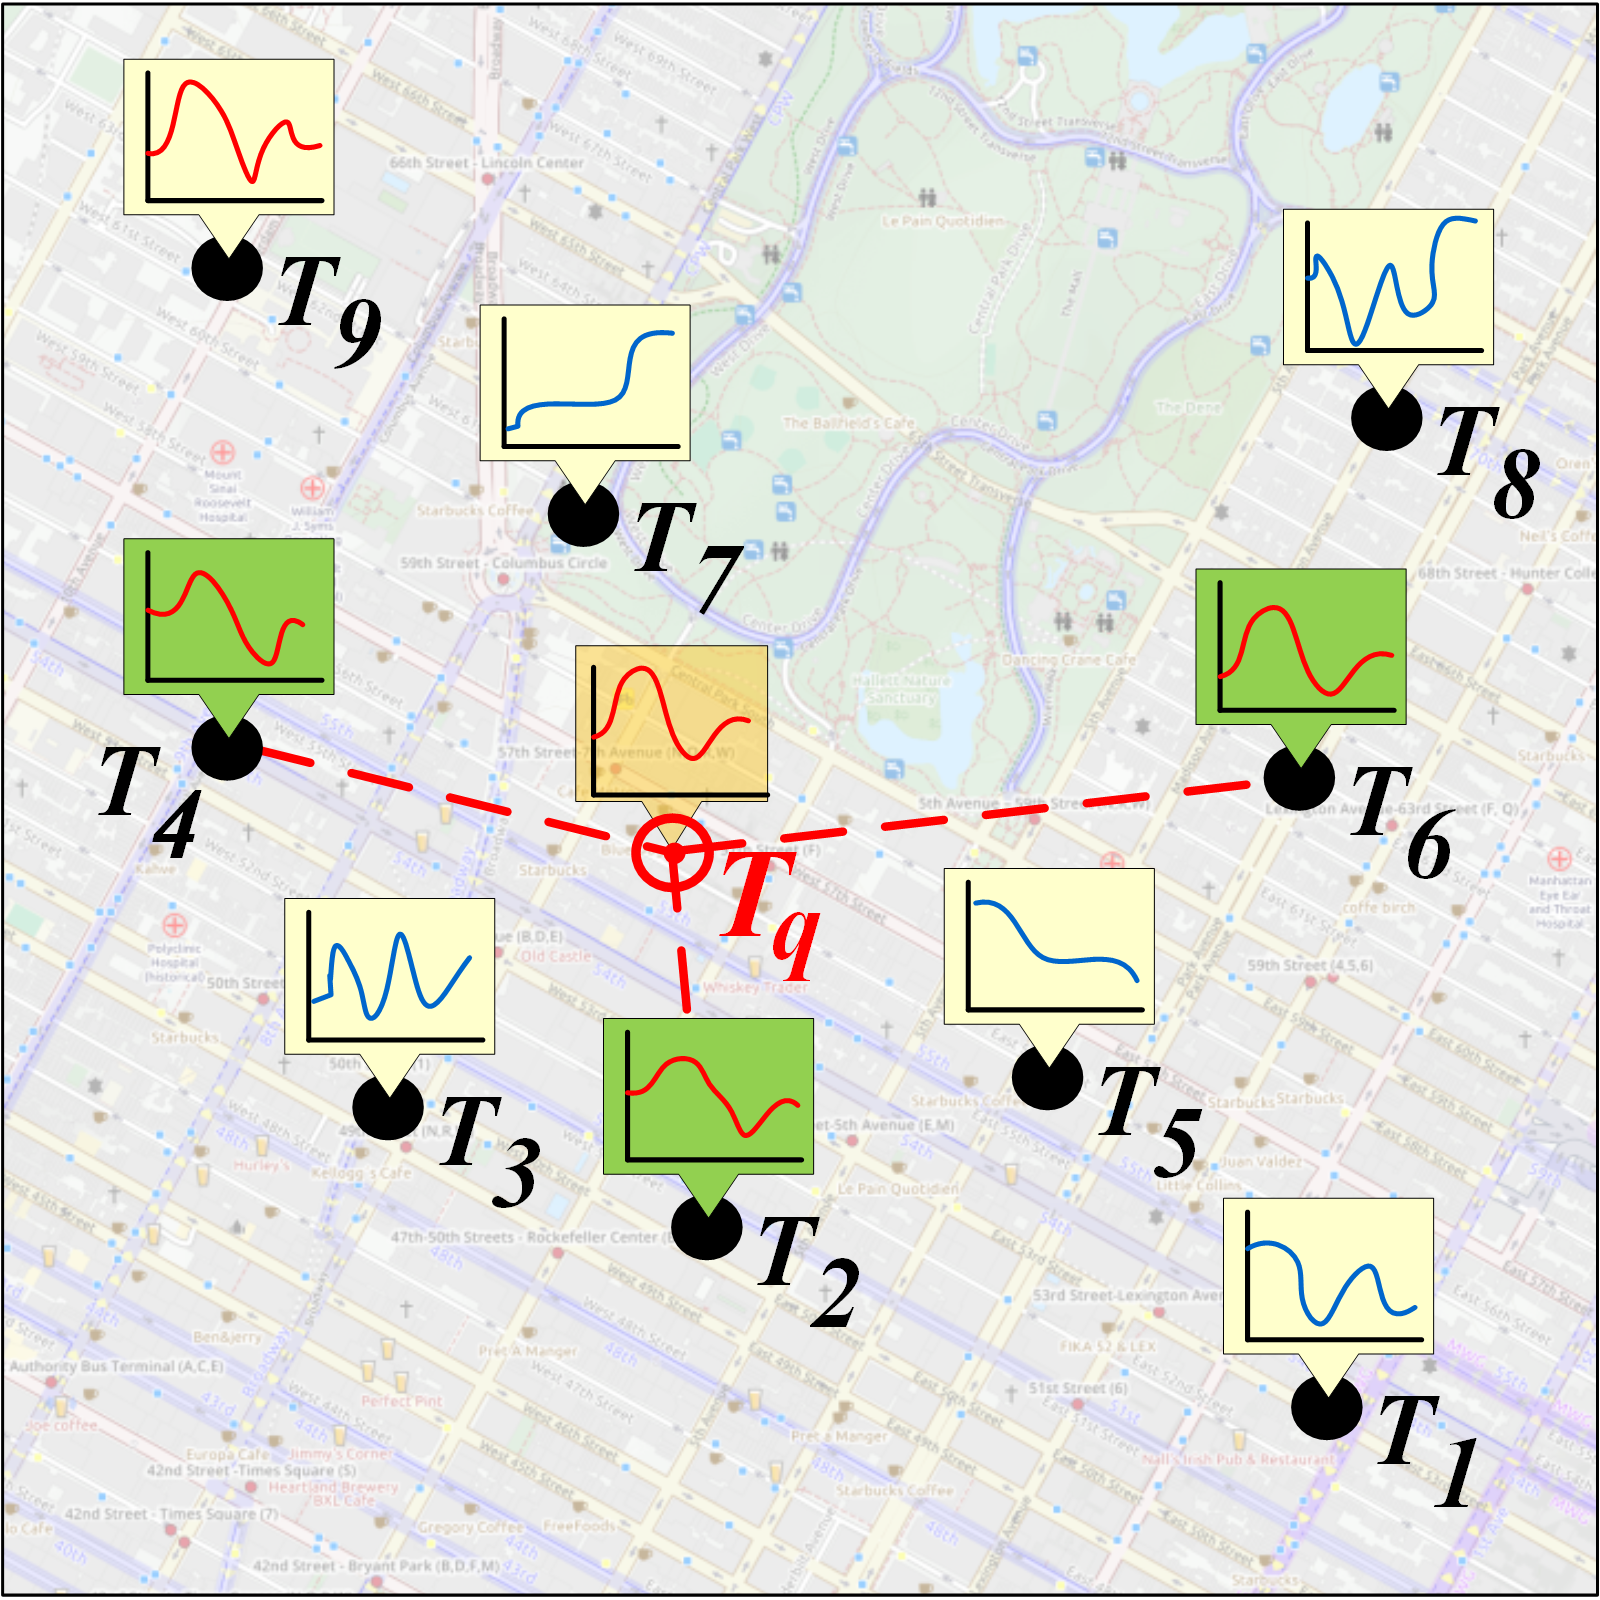
\includegraphics[width=0.3\textwidth]{figures/query_kb.png}\label{subfig:example_queries_kb}}
\caption{Hybrid queries on geolocated time series.}
\label{fig:example_queries}
\end{figure}

\begin{myexample}
 Figure \ref{fig:example_queries} illustrates an example including two queries, $Q_{bb}(T_q, \theta_{sp}, \theta_{ts})$ and $Q_{kb}(T_q, k, \theta_{ts})$, on a set of geolocated time series $T_1$, \ldots, $T_9$. In both cases, the reference time series $T_q$ specified by the query is shown in red. Moreover, those time series having dissimilarity to $T_q$ at most $\theta_{ts}$ (i.e., $T_2$, $T_4$, $T_6$, $T_9$) are also shown with red lines. In the first query, only time series within a radius equal to the spatial distance threshold $\theta_{sp}$ are retrieved. Thus, the result contains only time series $T_2$ and $T_4$, whereas $T_6$ and $T_9$ are excluded. The second query for $k=3$ retrieves the three closest time series to $T_q$ having dissimilarity at most $\theta_{ts}$, i.e., $T_2$, $T_4$ and $T_6$. \qed
\end{myexample}

\subsection{Similarity Join}
\label{subsec:sim_join_prob}
Contrary to similarity search, the hybrid similarity join query does not require an initial geolocated time series as reference. Given two datasets $R$ and $S$ (or just one dataset $S$ in the case of self-join), we seek all the existing pairs of geolocated time series that are close to each other both in terms of spatial and time series distance. Of course, both distance thresholds need to be provided before the query is executed. More formally:

\begin{mydefinition}[Hybrid Similarity Join over Geolocated Time Series]\label{def:sim_join}
  Given two sets of geolocated time series $\mathcal{T}_{R}$ and $\mathcal{T}_{S}$, and two thresholds $\epsilon_{sp}$ and $\epsilon_{ts}$, the {\em hybrid similarity join} query returns all pairs qualifying w.r.t. to both criteria on spatial proximity and time series similarity, i.e., 
  \[ \{ (T_{R}, T_{S}): T_{R} \in \mathcal{T}_{R}, T_{S} \in \mathcal{T}_{S}, dist_{sp}(T_{R}, T_{S})\leq\epsilon_{sp} \land dist_{ts}(T_{R}, T_{S}) \leq \epsilon_{ts} \}. \] 
\end{mydefinition} 
 
That is, this query searches for pairs of geolocated time series that are within spatial distance at most $\epsilon_{sp}$, while also their respective time series do not deviate by more than~$\epsilon_{ts}$. Spatial proximity is measured in distance units (e.g., meters). As mentioned before, since the (transformed) time series are $z$-normalized, values for parameter $\epsilon_{ts}$ are {\em unitless} and are typically expressed in standard deviations.
  
\begin{myexample}
Figure~\ref{fig:simjoin_example} depicts two sets of geolocated time series, $\{R_1, \dots, R_5\}$ (in red bullets) and $\{S_1, \dots, S_6\}$ (in green squares) that represent CO$_2$ emissions collected by two sensor networks $R$ and $S$ in an urban area during a day. Suppose that a similarity join query over those two datasets specifies a distance radius $\epsilon_{sp} = 500$ meters to identify nearby sensors and a maximum deviation of $\epsilon_{ts} = 0.4$ to find similar CO$_2$ patterns. Qualifying pairs  $\{ (R_1, S_5), (R_3, S_5),  (R_5, S_2) \}$ are shown connected with dashed lines. Note that other pairs, e.g., $(R_4, S_3)$, may be even closer in space, but their time series deviate more than the given $\epsilon_{ts}$, so they are filtered out. Besides, time series like those in rejected pair $(R_3, S_3)$ may have almost the same pattern, but their locations are too far from each other to qualify for this query.
\qed
\end{myexample}

\begin{figure}[!tb]
 \centering
 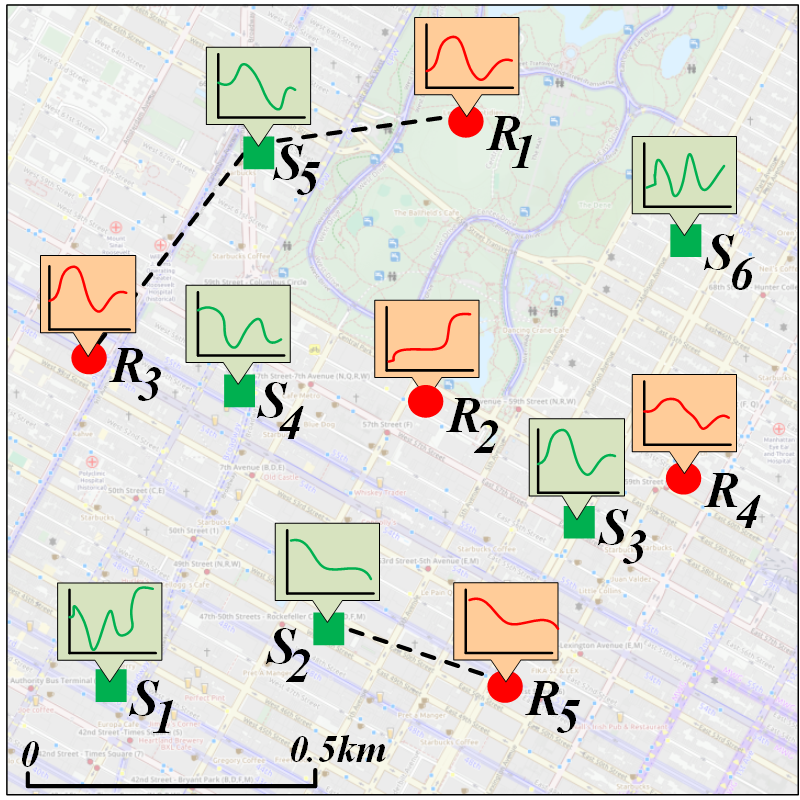
\includegraphics[width=0.33\textwidth]{figures/sim_join.png}
 \caption{Hybrid similarity join.}
\label{fig:simjoin_example}
\end{figure}